%!TEX root = Main.tex
\documentclass[Main]{subfiles}

\begin{document}

\section{Hardware} % (fold)
\label{sec:hardware}

	\subsection{Platform} % (fold)
	\label{sub:platform}

		The processing platform chosen for this project is a \emph{ZYBO Zynq™-7000 Development Board} from Digilent (see Figure \ref{fig:ZYBO}).
		The brains of the ZYBO is a Xilinx Zynq-7000 All Programmable System on a Chip (AP SoC).
		The AP SoC (see Figure \ref{fig:ZynqArch}) features both a Processing System (PS) consisting of 650 MHz dual core ARM\textregistered{} Cortex A9 CPU with dedicated I/O and Memory and extensible FPGA Programmable Logic (PL) for HW synthesis.

		This enables the construction of a system with software, written in C++, running on the CPU, and with dedicated hardware for acceleration of computation and I/O handling.
		\begin{figure}[H]
			\centering
			\begin{subfigure}[b]{0.55\linewidth}
				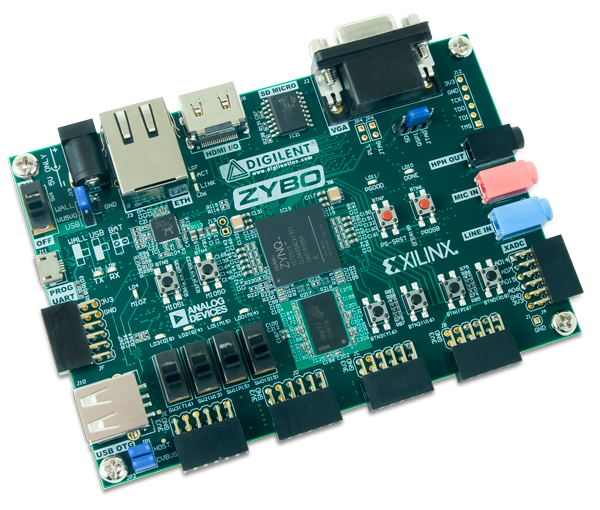
\includegraphics[width=\linewidth]{ZYBO}
				\caption{Digilent Zynq Board (ZYBO)}
				\label{fig:ZYBO}
			\end{subfigure}		
			\begin{subfigure}[b]{0.4\linewidth}
				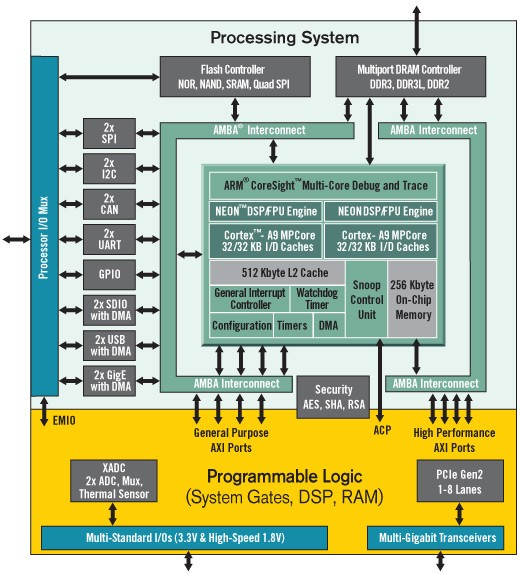
\includegraphics[width=\linewidth]{ZynqArch}
				\caption{Zynq-7000 AP SoC Diagram}
				\label{fig:ZynqArch}
			\end{subfigure}
			\caption{}		
		\end{figure}

		



		\subsubsection{HW/SW Co-Design} % (fold)
		\label{ssub:hw_sw_co_design}

			The availability of FPGA logic on-chip enables rapid prototyping of HW acceleration blocks, through the use of High-Level Synthesis (HLS) tools.
			Using HLS one can specify some desired functionality in C++/SystemC code and quickly synthesize it to HW-blocks to be implemented in FPGA logic.

			% subsubsection hw_sw_co_design (end)
	
		% subsection platform (end)

	\subsection{Power} % (fold)
	\label{sub:power}
	
	% subsection power (end)

	\subsection{Sensors} % (fold)
	\label{sub:sensor}
	
	% subsection sensor (end)

	\subsection{Motor Control} % (fold)
	\label{sub:motor_control}
	
	% subsection motor_control (end)


% section hardware (end)

\end{document}